\section{UbiquitOS}

\emph{Middleware} desenvolvido na Universidade de Brasília com foco na adaptabilidade de serviços~\cite{gomes2007} e cujo objetivo é prover serviços para seus usuários de maneira transparente, ou seja, sem que se perceba a influência de computação.

A figura~\ref{fig:ubiquitos} mostra uma visão do ecossistema do \emph{middleware} em que o \emph{uOS} coordena as aplicações e provê serviços por meio dos recursos (representados pelos \emph{drivers}) dos dispositivos presentes no ambiente. Os plugins de rede representam o meio de comunicação do \emph{uOS} com os dispositivos.

\begin{figure}[ht]
	\center
	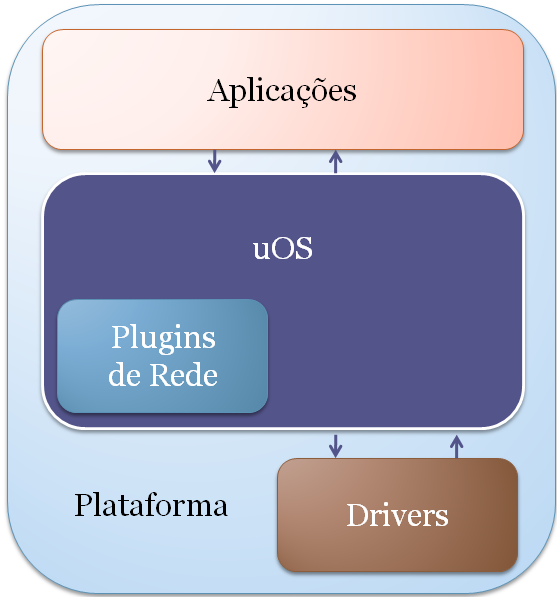
\includegraphics[scale=0.4]{imagens/ecossistemaUbiquitos}
	\caption{Ecossistema do \emph{middleware} UbiquitOS.}
	\label{fig:ubiquitos}
\end{figure}

\subsection{DSOA - \emph{Device Service Oriented Architecture}}

A DSOA foi definida baseada na arquitetura SOA(\emph{Service Oriented Architecture}). A SOA possui diversas características que podem auxiliar ambientes inteligentes, proporciona a capacidade da reutilização de recursos de software. Entretanto, por ser uma apenas uma arquitetura genérica, não leva em consideração características e limitações de ambientes inteligentes, descrevendo apenas serviços em alto nível e não define, ainda, um modelo de comunicação.

Na DSOA destacam-se cinco conceitos básicos:

\begin{itemize}
	\item Ambiente Inteligente:
		É um ambiente composto por pelo menos dois dispositivos capacidade de computação e conectados por meio de uma rede de comunicação coloborativa com os usuários do ambiente. O provimento de serviços para o usuário vem da interação das aplicações deste ambiente dinâmico. Essa dinamicidade do ambiente ubíquo se dá pelo fato que os usuários entram, saem e se movimentam no ambiente, além disso, trazem consigo seus dispositivos. É importante ressaltar que um ambiente inteligente neste trabalho não tem seu significado mais popular de ambiente com inteligência artificial.
	\item Dispositivo:
		É um aparelho que possua capacidade de comunicação e que abrigar aplicações ou disponibilizar seus recursos do ambiente inteligente para que outras aplicações possam utilizar de seus serviços.
	\item Recurso:
		É um grupo de funcionalidades relacionadas que podem ser acessadas por meio de interfaces pré-definidas.
		\begin{itemize}
			\item Interface do Recurso:
				O recurso é a entidade básica de interação entre dispositivos, visto que é por meio dele que as funcionalidades presentes no ambiente poderão ser acessadas. Para que isso possa é acontecer, é necessário que seja definida uma interface de comunicação que seja conhecida pelas entidades presentes no \emph{smart space}. Essa interface é constituída por dois elementos:
				\begin{itemize}
					\item Identificador:
						Responsável por identificar unicamente um recurso entre diversos recursos presentes no ambiente.
					\item Conjunto de serviços:
						Conjunto de serviços que constituem o recurso e são disponibilizados por ele.
				\end{itemize}
		\end{itemize}
	\item Serviço:
		É a implementação de uma funcionalidade disponibilizada para o ambiente pelo reucurso e uma interface conhecida.
		\begin{itemize}
			\item Interface do Serviço:
			\begin{itemize}
				\item Recurso:
					Recurso do qual o serviço faz parte. Os serviços são encontrados a partir dos recursos.
				\item Identificador:
					Responsável por identificar unicamente um serviço dentro do recurso.
				\item Parâmetros:
					Parâmetros que serão passados para o serviços realizar a funcionalidade requisitada.
			\end{itemize}
		\end{itemize}
	\item Aplicações:
		São as responsáveis pela implementação da inteligência do ambiente. As aplicações executam nos dispositivos presentes no ambiente e, a partir de informações providas pelos recursos do amibente, podem realizar ações. Elas interagem com o usuário intermediando suas ações junto ao ambiente. Elas funcionam se relacionando com recursos para notificar o usuário da alteração de algum estado, ou aguardam a execução de algum comando por parte do usuário.
\end{itemize}

\subsection{\emph{uP - Ubiquitous Protocols}}

É um conjunto de protocolos criados para estabelecer um meio de interação entre serviços levando em consideração a arquitetura DSOA. Esses protocolos definem o canal de comunicação e a forma de interação entre entidades do ambiente. As mensagens são transmitidas no formato JSON (\emph{JavaScript Object Notation}), que utiliza a codificação UTF-8, que foi escolhido por ser um formato estruturado, leve e independente de plataforma. O JSON foi utilizado ante o XML, pois possui menor tamanho de mensagens e esse fator pode ser decisivo em um ambiente com diversos dipositivos com capacidades computacionais diferentes. Dessa forma a limitação dos dispositivos é minimizada e exclui a necessidade de uma rede para tratamento dessas mensagens.

Cada um dos conceitos apresentados na DSOA possuem uma representação no \emph{uP} com seus respectivos atributos:

\begin{itemize}
	\item Dispositivo(\emph{UpDevice}):
	
		Por meio dos seguintes atributos, é possível identificar unicamente o dispositivo no ambiente, e quais são as interfaces rede que o dispositivo possui para realizar alguma comunicação:
		\begin{itemize}
			\item \emph{``name''}: 
			
			Identificador do dispositivo;
			\item \emph{``networks''}: 

			Lista de interfaces de rede do dispositivo. Cada interface é composta pelo tipo de rede e endereço do dispositivo.
		\end{itemize}
	\item \emph{Driver}(\emph{UpDriver}): 

		Representa o conceito do Recurso definido na DSOA. Como um dispositivo pode ter várias instâncias de um recurso, cada instância é identificada unicamente dentro do dispositivo que contém este recurso. O \emph{driver} é composto por:
		\begin{itemize}
			\item \emph{``name''}:

				Identificador do recurso no ambiente;
			\item \emph{``services''}:
				
				Lista de serviços síncronos do recurso;
			\item \emph{``events''}:
				
				Lista de serviços assíncronos do recurso.
		\end{itemize}
	\item Serviço(\emph{UpService}): 

		Representa o conceito de mesmo nome definido na DSOA. Sua interface é composta pelos seguintes atributos:
		\begin{itemize}
			\item \emph{``name''}:

				Identificador do serviço disponível no recurso;
			\item \emph{``parameters''}:
				
				Lista de parâmetros necessários para que o serviço seja executado. Esses parâmetros podem ser de dois tipos:
				\begin{enumerate}
					\item Opcional (\emph{OPTIONAL});
					\item Obrigatório (\emph{MANDATORY}).
				\end{enumerate}
		\end{itemize}
\end{itemize}

\subsubsection{Tipo de mensagens}

Para que possa haver interação entre as entidades no ambiente, o \emph{uP} especifica quatro tipos de mensagens e, caso exista necessidade,  podem ser personalizadas:

\begin{itemize}
	\item \emph{Service Call}: 

		Mensagem síncrona do \emph{uP}. Seus parâmetros são definidos por meio de suas propriedades, podendo ser obrigatórias ou opcionais:
		\begin{itemize}
			\item Obrigatórias:
				\begin{itemize}
					\item \emph{\bf{type}}: 

						Representa o tipo da mensagem. No caso desta mensagem, seu valor será \emph{``SERVICE\underline{ }CALL\underline{ }REQUEST''};
					\item \emph{\bf{driver}}: 

						Recurso do serviço requisitado;
					\item \emph{\bf{service}}:

						Nome do serviço requisitado;
					\item \emph{\bf{parameters}}:

						Contém os parâmetros do serviço.
				\end{itemize}
			\item Opcionais:
				\begin{itemize}
					\item \emph{\bf{instanceId}}:

						Representa o identificador único da instância do \emph{driver} do serviço requisitado;
					\item \emph{\bf{serviceType}}:
						
						Representa a forma de transmissão de dados;
					\item \emph{\bf{channelIDs}}:

						Representa os identificadores dos canais criados para a comunicação;
					\item \emph{\bf{channelType}}:

						Representa o tipo da rede utilizada na comunicação.
				\end{itemize}
		\end{itemize}
	\item \emph{Service Response}: 

		Mensagem que carrega dados da resposta dada pela execução de um serviço chamado pelo \emph{Service Call}. Essa mensagem possui as seguintes propriedades:
		\begin{itemize}
			\item \emph{\bf{type}}: 

				Representa o tipo da mensagem. No caso desta mensagem, seu valor será \emph{``SERVICE\underline{ }CALL\underline{ }RESPONSE''};
			\item \emph{\bf{responseData}}: 

				Parâmetro opcional que contem os dados da resposta da execução do serviço.
		\end{itemize}
	\item \emph{Notify}: 

		Similar ao \emph{Service Response}, porém carrega dados de notificações de eventos, ou seja, respostas de uma requisição assíncrona de um serviço. Suas propriedades são:
		\begin{itemize}
			\item \emph{\bf{type}}: 

				Representa o tipo da mensagem. No caso desta mensagem, seu valor será \emph{``NOTIFY''};
			\item \emph{\bf{driver}}: 

				Recurso do serviço requisitado;
			\item \emph{\bf{instanceId}}: 

				Representa o identificador da instância onde ocorreu evento;
			\item \emph{\bf{parameters}}: 

				Parâmetro opcional com informações sobre o evento.
		\end{itemize}
	\item \emph{Encapsulated Message}: 

		Utilizada para permitir mensagens codificadas. Esse tipo de mensagem possui as seguintes propriedades:
		\begin{itemize}
			\item \emph{\bf{type}}: 

				Representa o tipo da mensagem. No caso desta mensagem, seu valor será \emph{``ENCAPSULATED\underline{ }MESSAGE''};
			\item \emph{\bf{securityType}}: 

				Identificador do tipo de codificação utilizada;
			\item \emph{\bf{innerMessage}}: 

				Mensagem codificada.
		\end{itemize}
\end{itemize}

\subsubsection{Protocolos}

Com o objetivo de disponibilizar as características de visibilidade, interação e efeito, foram criados mecanismos de acesso aos recursos. O \emph{uP} é dividido em protocolos básicos, que são utilizados para invocar serviços e protocolos complementares que completam suas  funcionalidas.

\begin{itemize}
	\item Protocolos Básicos: 

		São divididos em SCP (\emph{Service Call Protocol}) e EVP(\emph{Event Protocol}). O primeiro possui arquitetura provedor-consumidor, ou seja, o consumidor requisita um serviço e o provedor retorna esse serviço para ele de forma síncrona. No último, o consumidor se registra em um evento no provedor, que response informando que o registro foi realizado com sucesso, e na ocorrência do evento, o consumidor é notificado pelo provedor, demonstrando uma forma assíncrona de comunicação.
	\item Protocolos Complementares:

		Além da interação entre os serviços provida pelos protocolos básicos, o \emph{uP} tem mecanismos que permitem que as aplicações obtenham informações sobre quais são os serviços disponíveis no ambiente e informações a respeito deles. Os protocolos são divididos em um grupo de protocolos com informações sobre o dispositivo e um grupo de protocolos com informações sobre o ambiente. Esses grupos são mapeados em um \emph{driver} que definem sua interface de comunicação. São protocolos complementares:
	\begin{itemize}
		\item \emph{Device Driver}: 

			Responsável por disponibilizar informações a respeito do dispositivo. Possui os seguintes serviços:
			\begin{itemize}
				\item \emph{ListDrivers}: 

					Provê uma lista de instâncias dos drivers disponíveis do dispositivo. Possui dois parâmetros opcionais:
					\begin{itemize}
						\item \emph{\bf{serviceName}}: 

							Nome do serviço;
						\item \emph{\bf{driverName}}: 

							Identificador do recurso.
					\end{itemize}
				\item \emph{Handshake}: 

					Neste protocolo, dois dispositivos trocam informações entre-si. O dispositivo que invoca esse serviço passa como parâmetro um objeto do tipo \emph{device} e recebe como retorno informações sobre o dispositivo que recebeu a chamada;
				\item \emph{Goodbye}: 

					Responsável por retirar o dispositivo da lista de dispositivos presentes no ambiente;
				\item \emph{Authenticate}: 

					Estabelece um contexto de segurança entre dois dispositivos por meio de um prévio compartilhamento de chaves.
			\end{itemize}
		\item \emph{Register Driver}: 

			Responsável por disponibilizar informações que um dispositivo possui sobre o ambiente.
			\begin{itemize}
				\item \emph{ListDrivers}: 

					Provê uma lista de instâncias dos drivers disponíveis no ambiente, geralmente de dispositivos vizinhos. Possui três parâmetros opcionais:
					\begin{itemize}
						\item \emph{\bf{serviceName}}: 

							Nome do serviço;
						\item \emph{\bf{driverName}}: 

							Identificador do recurso;
						\item \emph{\bf{device}}: 
							
							Nome do dispositivo que contém o recurso.
					\end{itemize}
				\item \emph{Publish}: 

					Responsável pela publicação de uma instância de um driver a ser disponibilizada no ambiente.
				\item \emph{UnPublish}: 

					Responsável por retirar as informações sobre uma instância de um driver.
			\end{itemize}
	\end{itemize}
\end{itemize}

